\documentclass[11pt]{homework}

% TODO: replace these with your information
\newcommand{\hwname}{傅申}
\newcommand{\hwid}{PB20000051}
\newcommand{\hwtype}{计算机组成原理作业}
\newcommand{\hwnum}{1}

\usepackage{float}
\usepackage{graphicx}
\usepackage{amsfonts}

\newcommand{\overbar}[1]{\mkern 1.5mu\overline{\mkern-1.5mu#1\mkern-1.5mu}\mkern 1.5mu}

\begin{document}
\maketitle
% Your content
\question
式 a 可以化为
\begin{align}
    \begin{aligned}
        E &= ((A\cdot B)+(A\cdot C)+(B\cdot C))\cdot(\overbar{A\cdot B\cdot C})\\
          &= ((A\cdot B)+(A\cdot C)+(B\cdot C))\cdot(\overbar{A}+\overbar{B}+\overbar{C})\\
          &= (A\cdot B)\cdot(\overbar{A}+\overbar{B}+\overbar{C})+(A\cdot C)\cdot(\overbar{A}+\overbar{B}+\overbar{C})+(B\cdot C)\cdot(\overbar{A}+\overbar{B}+\overbar{C})\\
          &= (A\cdot B)\cdot \overbar{C}+(A\cdot C)\cdot\overbar{B}+(B\cdot C)\cdot\overbar{A}\\
          &= (A\cdot B\cdot \overbar{C})+(A\cdot C\cdot\overbar{B})+(B\cdot C\cdot\overbar{A})
    \end{aligned}
\end{align}
即为式 b.
\question
记四输入分布为 $A, B, C, D$, 输出为 $L$, 则显然有 $L=A\oplus B\oplus C\oplus D$ ($\oplus$ 代表异或), 即

\begin{equation}
    L=A\oplus B\oplus C\oplus D=(A\overbar{B}+\overbar{A}B)\oplus (C\overbar{D}+\overbar{C}D)=E\overbar{F}+\overbar{E}F
\end{equation}

其中 $E = A\overbar{B}+\overbar{A}B, F = C\overbar{D}+\overbar{C}D$. 对应的电路图如下.

\begin{figure}[!htbp]
    \centering
    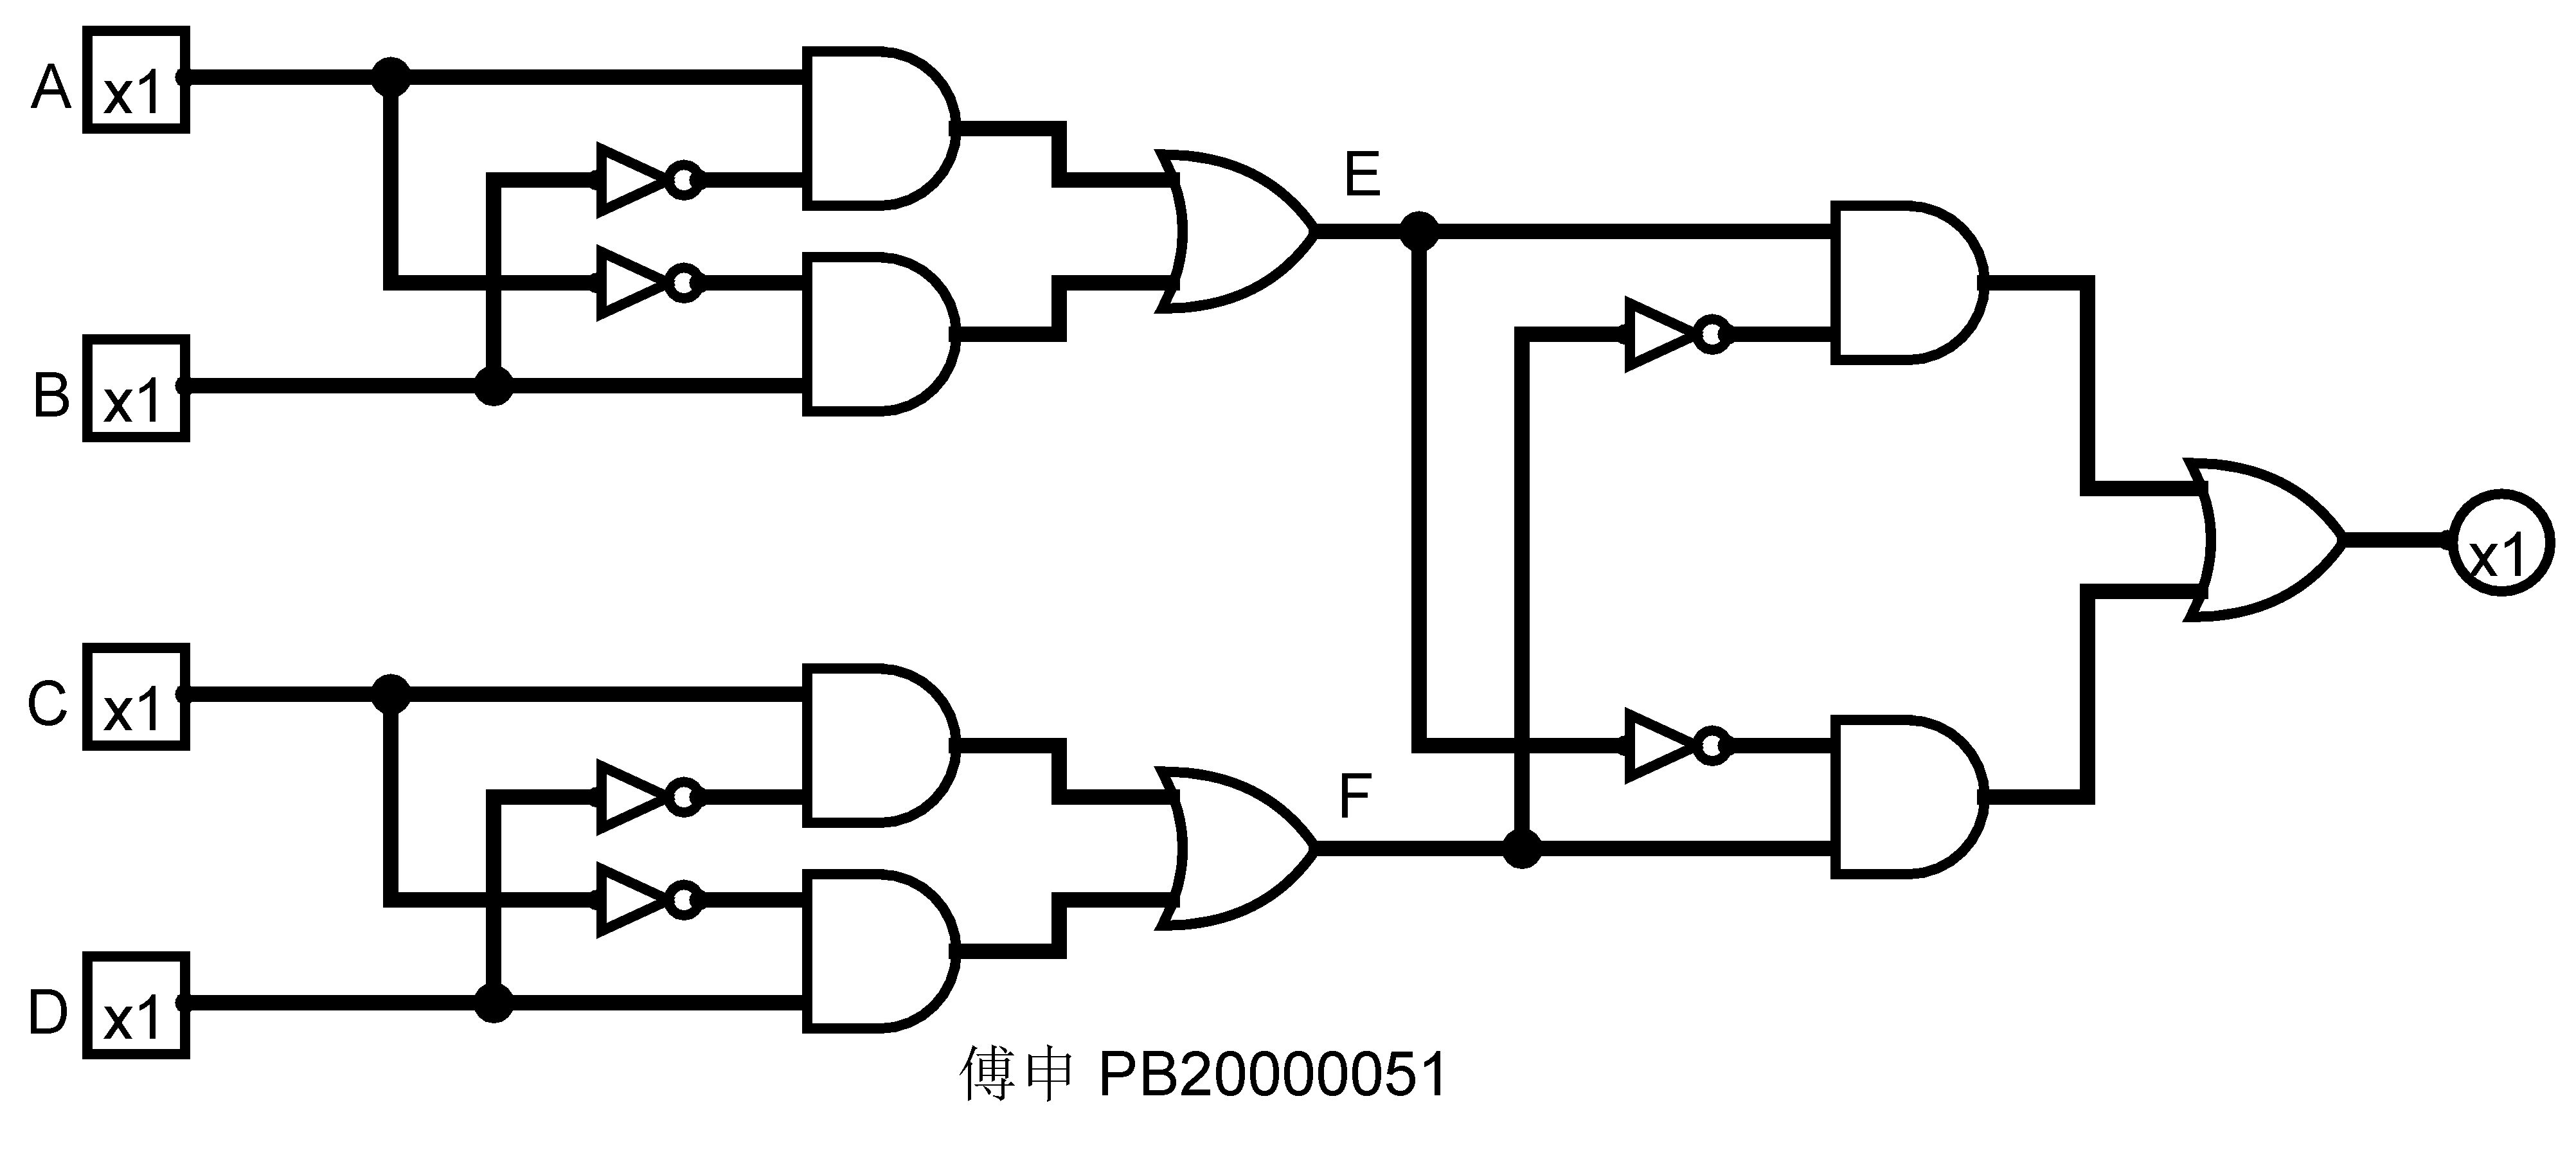
\includegraphics[width=.6\textwidth]{images/fig_1.png}
    \caption{奇校验函数电路图}
\end{figure}
\question
\begin{enumerate}[label = \alph*)]
    \item 
    \begin{itemize}
        \item $L_1=x_2x_1\overbar{x_0}+x_2\overbar{x_1}x_0+\overbar{x_2}x_1x_0$
        \item $L_2=x_2\overbar{x_1}\overbar{x_0}+\overbar{x_2}x_1\overbar{x_0}+\overbar{x_2}\overbar{x_1}x_0$
        \item $L_3=\overbar{x_2}$
        \item $L_4=x_2$
    \end{itemize}
    \item 按顺序如下
    \begin{figure}[!htbp]
        \centering
        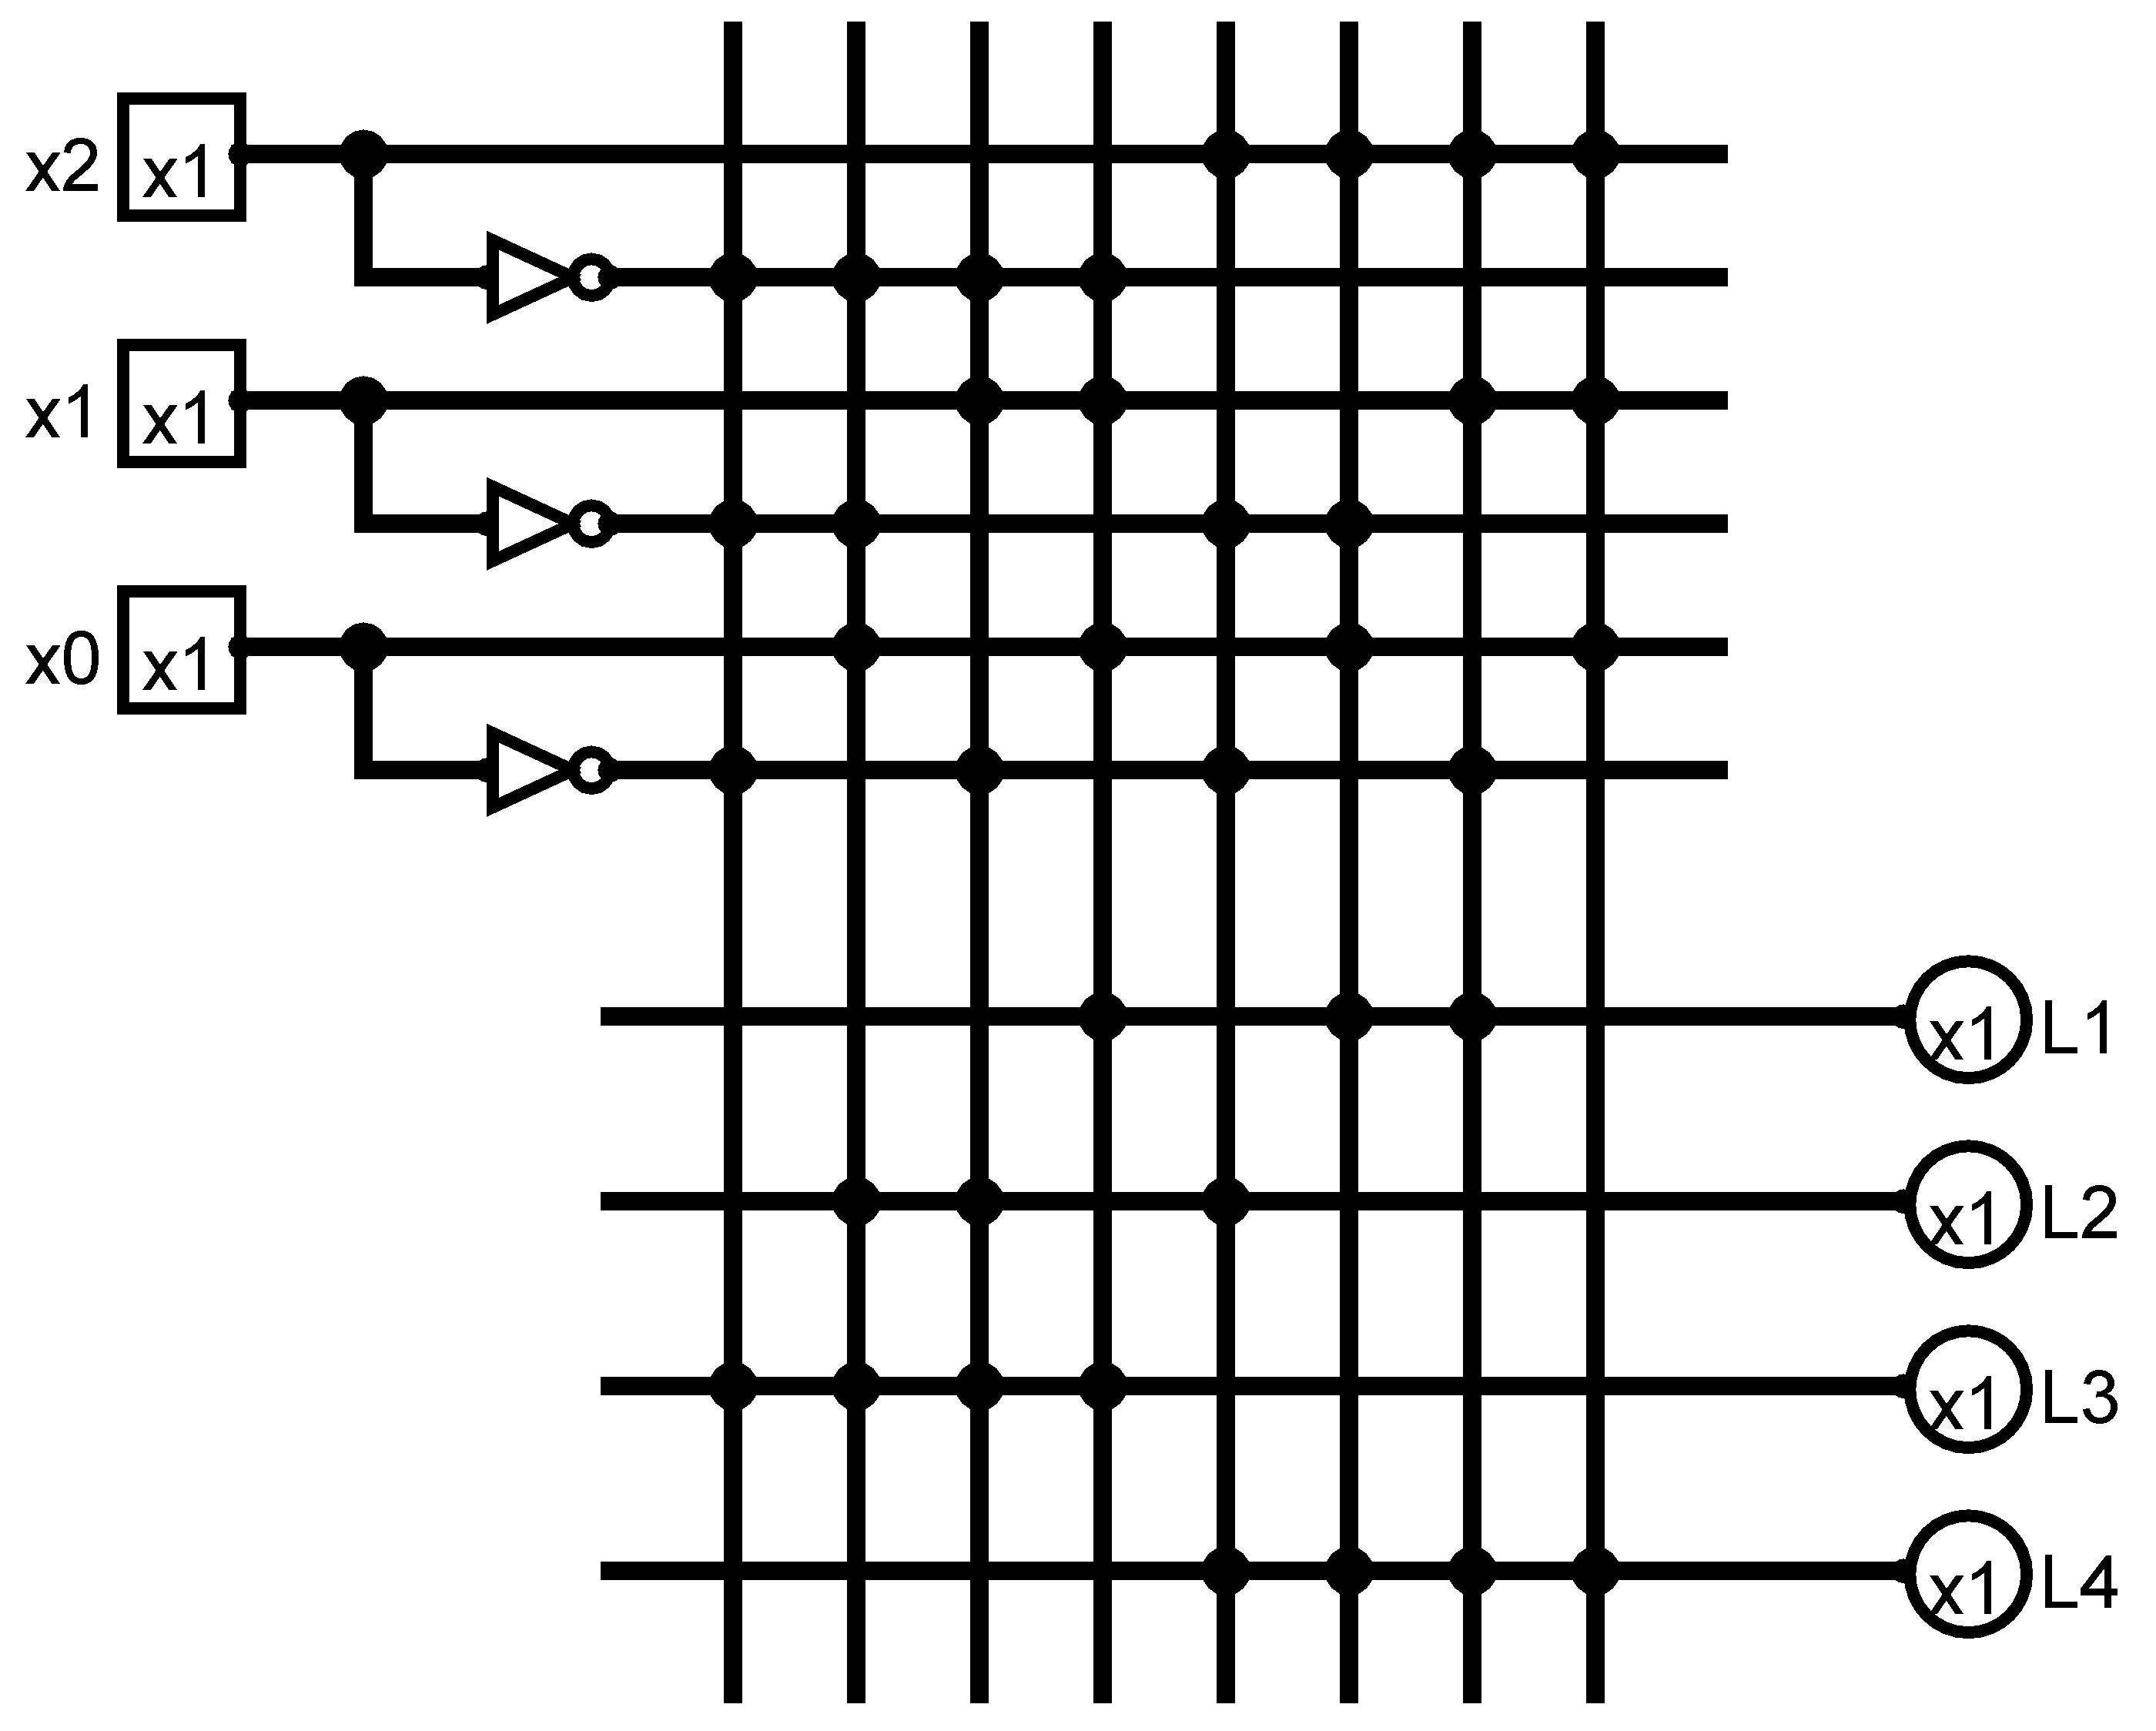
\includegraphics[width = .6\textwidth]{images/fig_2.png}
        \caption{PLA 实现}
    \end{figure}

\end{enumerate}
\question
\begin{itemize}
    \item \texttt{FUNC1} 实现了一个两输入多选器 (MUX), 当 \texttt{S} 为高电平时输出 \texttt{I1}, 否则输出 \texttt{I0}.
    \item \texttt{FUNC2} 实现了一个 8 位计数器, 若 \texttt{ctl} 为高电平则正向计数 (递增), 否则反向计数 (递减), 在时钟上沿计数, \texttt{rst} 为高电平时清零.
\end{itemize}
\question
\begin{lstlisting}[language=Verilog]
module adder (
    input [3:0] in4,
    input [15:0] in16,
    output [15:0] out
);
    assign out = {12'h000, in4} + in16;
endmodule
module register (
    input clk,
    input rst,
    input [15:0] in,
    input load_en,
    input [15:0] load,
    output [15:0] out 
);
    reg [15:0] regfile;
    always @(posedge clk or posedge rst) begin
        if (rst) regfile <= 16'h0000;
        else if (load_en) regfile <= load;
        else regfile <= in;
    end
endmodule
module main (
    input [3:0] in,
    input [15:0] LOAD,
    input Clk,
    input Rst,
    input Load,
    output [15:0] Out 
);
    wire [15:0] bus;
    wire [15:0] adder_out;
    assign out = bus;
    adder Adder(
        .in4(in), 
        .in16(bus), 
        .out(adder_out)
    );
    register Register(
        .clk(Clk), 
        .rst(Rst), 
        .in(adder_out),
        .load_en(Load), 
        .load(LOAD), 
        .out(bus)
    );
endmodule
\end{lstlisting}
\end{document}
